\documentclass[12pt,a4paper]{report}

\usepackage[a4paper,margin=1in]{geometry}
\usepackage[utf8]{inputenc}
\usepackage[T1]{fontenc}
\usepackage{lmodern}
\usepackage{graphicx}
\usepackage{booktabs}
\usepackage{tabularx}
\usepackage{enumitem}
\usepackage{setspace}
\usepackage{tikz}
\usetikzlibrary{arrows.meta,positioning}
\usepackage[hidelinks]{hyperref}

\onehalfspacing

\begin{document}

% TITLE PAGE
\begin{titlepage}
    \begin{center}
        {\LARGE \textbf{MUMBAI UNIVERSITY}}\\[0.4cm]
        {\Large \textbf{ST.\ FRANCIS INSTITUTE OF TECHNOLOGY}}\\[0.3cm]
        {\large Department of Computer Engineering}\\[1.8cm]

        {\Large \textbf{NLP MINI PROJECT REPORT}}\\[1.3cm]

        {\Huge \textbf{Konkan Vani}}\\[0.4cm]
        {\large (Konkani Vani)}\\[0.7cm]
        {\large \textbf{A Bilingual Konkani Idiom and Proverb Meaning Retrieval System}}\\[1.2cm]

        Submitted in partial fulfillment of the requirements for\\
        Bachelor of Engineering in Computer Engineering\\[1.2cm]

        {\large \textbf{Submitted by}}\\[0.3cm]
        \begin{tabular}{ll}
            SIDDANT SAWANT & 26\\
            KSHITIJ SHARMA & 32\\
            KRISHNA SHARMA & 31\\
        \end{tabular}\\[0.9cm]

        ..\\[0.2cm]
        {\large \textbf{Project Guide}}\\[0.2cm]
        {\large PRADNYA SAWANT}\\[0.9cm]

        ..\\[0.4cm]
        {\large 2026--2027}
    \end{center}
\end{titlepage}

\pagenumbering{roman}

\chapter*{Certificate}
\addcontentsline{toc}{chapter}{Certificate}
This is to certify that the mini project report entitled ``Konkan Vani: A Bilingual
Konkani Idiom and Proverb Meaning Retrieval System'' is submitted by
[STUDENT NAME(S)] of [DEPARTMENT / CLASS] at [COLLEGE NAME] during the academic
year [YEAR]. The work is presented in partial fulfillment of the requirements for
[COURSE / DEGREE].

\vspace{2cm}
\noindent
\begin{tabularx}{\textwidth}{XX}
    \textbf{Project Guide:} & \textbf{Head of Department:}\\[2cm]
    \textbf{Date:} & \textbf{Place:}\\
\end{tabularx}
\clearpage

\chapter*{Declaration}
\addcontentsline{toc}{chapter}{Declaration}
We declare that the project entitled ``Konkan Vani: A Bilingual Konkani Idiom and
Proverb Meaning Retrieval System'' has been prepared by us for the NLP Mini
Project. The report should be submitted only after all descriptions,
implementation details, dataset provenance, and results have been checked against
the actual project files and test outputs. Any external material used will be
acknowledged and cited according to the college's requirements.

\vspace{1cm}
\noindent \textbf{Student signatures:}\\[0.3cm]
\textbf{Names:} siddant sawant, krishna sharma, kshitij sharma\\[0.5cm]
\textbf{Date:}
\clearpage

\chapter*{Acknowledgement}
\addcontentsline{toc}{chapter}{Acknowledgement}
We express our gratitude to [PROJECT GUIDE NAME] for guidance and feedback during
the development of this mini project. We also thank the Department of
[DEPARTMENT NAME], [COLLEGE NAME], for providing the opportunity to study natural
language processing through a practical application. We acknowledge the authors
and maintainers of the open-source tools and models used in the project, including
Next.js, FastAPI, SentenceTransformers/LaBSE, FAISS, and RapidFuzz. This section
should be revised to reflect the actual people and resources that supported the
work.
\clearpage

\chapter*{Abstract}
\addcontentsline{toc}{chapter}{Abstract}
Konkan Vani is a web-based natural language processing (NLP) project designed to
help users retrieve meanings of Konkani idioms and proverbs. The proposed workflow
accepts queries in forms such as Devanagari Konkani, Romanized Konkani,
Kannada-script transliterations, and English or Marathi descriptions. A web client
built with Next.js communicates with a Python FastAPI service. The retrieval
pipeline is described as a staged process: phonetic and fuzzy matching with
RapidFuzz, multilingual semantic retrieval using LaBSE sentence embeddings and a
FAISS vector index, and a fallback response mechanism for queries that do not meet
the matching thresholds.

The README supplied for this report describes a dataset of 5,200 idiom entries,
768-dimensional embeddings, and a vector index used for similarity search. It also
reports benchmark cases for exact-script queries, Romanized spelling variants,
semantic retrieval, and out-of-domain rejection. These dataset counts,
implementation details, and performance results must be verified against the
repository, dataset provenance, and reproducible test logs before final
submission. The project aims to support access to linguistic and cultural
meanings through a searchable bilingual interface.

\vspace{0.5cm}
\noindent \textbf{Keywords:} Natural Language Processing, Konkani, idiom
retrieval, multilingual embeddings, LaBSE, FAISS, RapidFuzz, semantic search.
\clearpage

\tableofcontents
\listoffigures
\listoftables
\clearpage

\pagenumbering{arabic}

\chapter{Introduction}

\section{Background}
Natural Language Processing enables computer systems to process, compare, and
retrieve information expressed in human language. Idioms and proverbs are
challenging because their intended meanings often differ from literal word-by-word
interpretations. Their spelling may also vary when users write a language in
different scripts or use informal transliteration.

Konkani is used across communities and may be written in more than one script. A
search tool that handles spelling variation and meaning similarity can make
idiomatic expressions easier to explore and understand. Konkan Vani is designed as
a web portal for searching Konkani idioms and presenting literal, figurative,
English, and Marathi meanings where the dataset provides them.

\section{Problem Statement}
Users may struggle to find the meaning of a Konkani idiom when they do not know
its exact spelling, when they enter a Romanized form, or when they describe the
meaning in another language. A simple exact-string search may fail to retrieve the
intended expression. The project addresses this problem through a combination of
fuzzy matching and multilingual semantic retrieval.

\section{Objectives}
\begin{enumerate}
    \item Develop a web interface for searching and browsing Konkani idioms and
          proverbs.
    \item Support multiple query forms and script representations as implemented
          by the application.
    \item Combine phonetic/fuzzy matching with semantic vector retrieval.
    \item Present structured meaning fields such as literal meaning, figurative
          meaning, English meaning, Marathi meaning, and example sentences when
          available.
    \item Evaluate representative matching and out-of-domain query behaviour using
          reproducible tests.
\end{enumerate}

\section{Scope}
The scope described in the project README includes a web frontend, a FastAPI
backend, a curated idiom dataset, phonetic normalization, sentence embeddings,
vector similarity search, and a fallback mechanism. The quality and breadth of
language coverage depend on the dataset and must not be generalized beyond what
the available data supports.

\section{Organization of the Report}
Chapter 1 introduces the project. Chapter 2 reviews relevant concepts and related
approaches. Chapter 3 presents requirements and system design. Chapter 4 describes
the methodology and implementation. Chapter 5 presents testing and results.
Chapter 6 concludes the report and discusses future work.

\chapter{Literature Survey and Technical Background}

\section{Natural Language Processing}
NLP combines computational methods and linguistic information to support tasks
such as text normalization, classification, translation, and information
retrieval. For this project, the central task is retrieval: given a query, identify
a relevant idiom record and return its associated meanings.

\section{Fuzzy String Matching}
Fuzzy matching estimates similarity between strings rather than requiring exact
equality. RapidFuzz provides efficient string-similarity functions. The README
describes use of token sort ratio with a stated cutoff of 75\%. The exact
normalization and scoring behaviour should be checked in the implementation before
being described as a final design decision.

\section{Multilingual Sentence Embeddings}
Sentence embeddings represent text as numerical vectors so that semantically
similar text can be compared geometrically. The project README identifies the
SentenceTransformers model \texttt{sentence-transformers/LaBSE} and describes
768-dimensional vectors. Model versions, preprocessing, and vector normalization
should be documented from the actual build scripts.

\section{Vector Similarity Search with FAISS}
FAISS is a library for efficient similarity search over dense vectors. The README
describes an IndexFlatIP index and a cosine-similarity threshold of 0.55. Inner
product corresponds to cosine similarity only when vectors are appropriately
normalized; verify that the embedding/index-building code normalizes vectors
before making this claim in the final report.

\section{Web Application Frameworks}
Next.js supports the client-facing web application, while FastAPI exposes Python
endpoints for health checks, search, browsing, statistics, and resolution. The
frontend/backend separation enables the interface and NLP logic to be developed
and tested independently.

\section{Summary}
The described system combines lexical similarity and semantic retrieval. This
hybrid approach can address both spelling variation and queries whose wording
differs from the stored idiom. The system should also reject unrelated queries
when confidence is insufficient.

\chapter{Requirements and System Design}

\section{Functional Requirements}
\begin{enumerate}[label=FR\arabic*.]
    \item The user can enter a query for an idiom or phrase.
    \item The application can return matching idiom records and available meaning
          fields.
    \item The user can browse records with supported filters and pagination.
    \item The system exposes health and statistics endpoints, if enabled in the
          running build.
    \item The system can indicate no reliable match for unsupported or
          out-of-domain queries.
\end{enumerate}

\section{Non-Functional Requirements}
\begin{itemize}
    \item \textbf{Usability:} the interface should be understandable and
          responsive.
    \item \textbf{Maintainability:} frontend, backend, data preparation, and
          indexing code should remain modular.
    \item \textbf{Reliability:} missing data or unavailable services should be
          handled gracefully.
    \item \textbf{Performance:} retrieval latency should be measured under a
          documented test setup.
    \item \textbf{Reproducibility:} model, dataset, dependency versions, and build
          steps should be recorded.
\end{itemize}

\section{System Architecture}
The architecture described in the README contains a Next.js frontend communicating
with a FastAPI backend over HTTP. The backend loads the idiom records and the
vector index, then applies a staged resolver.

\begin{figure}[ht]
    \centering
    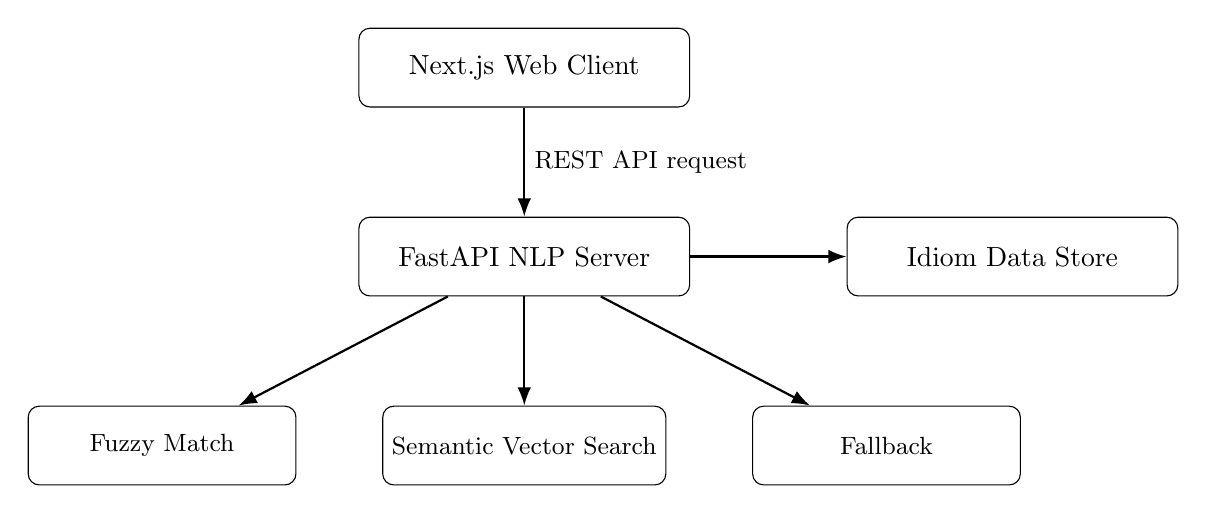
\begin{tikzpicture}[
        box/.style={draw, rounded corners, minimum width=4.2cm, minimum height=1cm, align=center},
        stage/.style={draw, rounded corners, minimum width=3.4cm, minimum height=1cm, align=center, font=\small},
        arrow/.style={-{Latex}, thick}
    ]
        \node[box] (client) at (0,0) {Next.js Web Client};
        \node[box] (api) at (0,-2.4) {FastAPI NLP Server};
        \node[box] (store) at (6.2,-2.4) {Idiom Data Store};
        \node[stage] (fuzzy) at (-4.6,-4.8) {Fuzzy Match};
        \node[stage] (semantic) at (0,-4.8) {Semantic Vector Search};
        \node[stage] (fallback) at (4.6,-4.8) {Fallback};

        \draw[arrow] (client) -- node[right, font=\small] {REST API request} (api);
        \draw[arrow] (api) -- (store);
        \draw[arrow] (api) -- (fuzzy);
        \draw[arrow] (api) -- (semantic);
        \draw[arrow] (api) -- (fallback);
    \end{tikzpicture}
    \caption{High-level architecture of Konkan Vani. Replace this placeholder with
    a polished diagram if required.}
    \label{fig:architecture}
\end{figure}

\section{Major Modules}

\begin{table}[ht]
    \centering
    \begin{tabularx}{\textwidth}{p{3.8cm}X}
        \toprule
        \textbf{Module} & \textbf{Responsibility described in the README}\\
        \midrule
        Frontend & Search, browse, script selection, and result presentation.\\
        API client & Sends requests to the backend and includes a fallback
                     mechanism as described in the README.\\
        FastAPI server & Provides HTTP endpoints for search, resolution, browsing,
                         statistics, and health.\\
        Phonetic normalization & Normalizes supported text forms to help compare
                                 spelling variants.\\
        Query pipeline & Orchestrates fuzzy matching, semantic search, and fallback
                         handling.\\
        Embedding builder & Encodes idiom text into dense vectors using the
                            configured sentence-embedding model.\\
        FAISS index builder & Creates the similarity-search index and associated
                              metadata.\\
        \bottomrule
    \end{tabularx}
    \caption{Major modules and their responsibilities.}
    \label{tab:modules}
\end{table}

\section{Hardware and Software Requirements}
The README specifies Python 3.10 or higher and Node.js 18 or higher, with example
verification on Python 3.12.5 and Node.js 22.16.0. Record the actual versions used
during testing. Hardware requirements, operating system, RAM, and whether a GPU
was used should be filled in from the actual test environment.
\chapter{Methodology and Implementation}

\section{Data Preparation}
The README identifies a processed CSV file named \texttt{idioms with phonetic
keys.csv} and describes 5,200 records with fields for the Konkani expression,
Romanized form, script, meanings, example sentence, category, cultural context,
phonetic key, and source. The dataset's provenance, licensing, translation
accuracy, and human-review process should be documented. Do not claim expert
validation unless evidence is available.

\section{Phonetic Normalization and Fuzzy Matching}
In the first stage, the system normalizes the input and compares it with stored
phonetic keys or text variants. The README states that RapidFuzz's token sort
ratio is used with a 75\% cutoff. The code should be inspected to confirm the
exact sequence of normalization, candidate selection, score interpretation, and
handling of ties.

\section{Semantic Retrieval}
If fuzzy matching does not return a sufficiently confident result, the described
pipeline encodes the query with LaBSE and compares it with precomputed idiom
vectors in FAISS. The README specifies a 768-dimensional embedding space and a
stated cutoff of 0.55. Confirm vector normalization, model loading, index metric,
and threshold logic from the implementation.

\section{Fallback Handling}
The README describes a fallback generator for queries that do not pass the earlier
stages. Explain in the final report whether the fallback returns a generic
explanation, a generated response, or a no-match message, based on the actual
code. Clearly distinguish generated explanations from verified dataset entries.

\section{API Endpoints}
The README documents the following endpoints. Confirm the route definitions and
response schemas in the source before submission.

\begin{table}[ht]
    \centering
    \begin{tabularx}{0.85\textwidth}{lX}
        \toprule
        \textbf{Endpoint} & \textbf{Purpose}\\
        \midrule
        \texttt{GET /health} & Reports server health and index status.\\
        \texttt{GET /api/search} & Performs query-based idiom retrieval.\\
        \texttt{GET /api/browse} & Returns paginated records with supported filters.\\
        \texttt{GET /api/stats} & Returns dataset/index statistics.\\
        \texttt{POST /api/resolve} & Performs lower-level query resolution.\\
        \bottomrule
    \end{tabularx}
    \caption{Documented API endpoints.}
    \label{tab:endpoints}
\end{table}

\section{Running the Application}
According to the README, setup involves installing Python dependencies, generating
or checking the dataset, building embeddings and the FAISS index when required,
starting the FastAPI server, and running the Next.js client with \texttt{npm
install} and \texttt{npm run dev}. The final report should include only the steps
that were actually run successfully by the project team. Do not rebuild large
embeddings unnecessarily if the required artifacts are already present and
verified.

\chapter{Testing and Results}

\section{Testing Strategy}
Testing should cover exact-script queries, Romanized spellings, spelling variants,
semantically phrased queries, out-of-domain queries, API health, and
frontend/backend integration. Record the test environment, query set, expected
output, actual output, and pass/fail status.

\section{Results Reported in the README}
The README reports the following example checks. These are project-reported
results and must be reproduced from test logs before being presented as
independently verified results.

\begin{table}[ht]
    \centering
    \begin{tabularx}{\textwidth}{p{3.2cm}p{3.4cm}p{3.4cm}p{2.6cm}}
        \toprule
        \textbf{Query type} & \textbf{Reported outcome} & \textbf{Reported stage} & \textbf{README status}\\
        \midrule
        Exact Devanagari idiom & Expected idiom returned & Semantic vector & Pass\\
        Romanized spelling variant & Expected idiom returned & Phonetic fuzzy & Pass\\
        Phonetic variant & Expected idiom returned & Phonetic fuzzy & Pass\\
        Unrelated English query & Rejected & Threshold filter & Pass\\
        Out-of-domain Devanagari query & Rejected & Threshold filter & Pass\\
        \bottomrule
    \end{tabularx}
    \caption{Benchmark cases as reported in the README.}
    \label{tab:results}
\end{table}

\section{Performance Metrics}
The README states approximate stage timings of 1--3\,ms for fuzzy matching and
15--25\,ms for semantic search. These values require repeatable measurement with a
defined machine, warm/cold model state, batch size, and timing method. Report
mean/median and percentile latency if a sufficiently large test run is available.

\section{Limitations}
Potential limitations to investigate include coverage and accuracy of the idiom
dataset, script/transliteration ambiguity, threshold sensitivity, dialect
variation, quality of automatically expanded records, dependence on model
downloads and index files, and the risk of fallback text being mistaken for a
verified translation. Include only limitations relevant to the actual
implementation and testing.

\chapter{Conclusion and Future Scope}

\section{Conclusion}
Konkan Vani is designed as a hybrid retrieval system for Konkani idioms and
proverbs. Its described architecture combines a web interface, a Python API,
phonetic fuzzy matching, multilingual sentence embeddings, vector similarity
search, and fallback handling. The approach aims to improve retrieval when users
enter variant spellings or describe an idiom's meaning rather than reproducing its
exact stored form. Final conclusions should be based on verified code, dataset
checks, and repeatable tests.

\section{Future Scope}
The README proposes GPU acceleration for larger collections, text-to-speech
pronunciation support, and a community contribution/review dashboard. Other
possible improvements include expert review of idiom meanings, transparent
provenance for each entry, broader dialect coverage, and a benchmark set annotated
by fluent speakers.

\chapter*{References}
\addcontentsline{toc}{chapter}{References}
\begin{enumerate}
    \item Hugging Face, ``LaBSE model documentation'',
          \url{https://huggingface.co/sentence-transformers/LaBSE}. Accessed:
          [DATE].
    \item Facebook AI Research, ``FAISS documentation'',
          \url{https://github.com/facebookresearch/faiss}. Accessed: [DATE].
    \item RapidFuzz, ``RapidFuzz documentation'',
          \url{https://rapidfuzz.github.io/RapidFuzz/}. Accessed: [DATE].
    \item FastAPI, ``FastAPI documentation'', \url{https://fastapi.tiangolo.com/}.
          Accessed: [DATE].
    \item Vercel, ``Next.js documentation'', \url{https://nextjs.org/docs}.
          Accessed: [DATE].
\end{enumerate}

\appendix
\chapter{Screenshots and Evidence}
Insert actual screenshots of the home/search page, successful query result,
Romanized query, no-match query, browse page, API health response, and test
output. Give each figure a number and caption. Do not use illustrative screenshots
as evidence of a working implementation.

\chapter{Reproducibility Checklist}
\begin{itemize}
    \item Confirm the dataset file exists and document its source.
    \item Confirm model and FAISS index dimensions/counts from scripts or output.
    \item Run the test suite and save the actual output.
    \item Test the frontend with the backend running.
    \item Record software versions and hardware.
    \item Replace all bracketed placeholders.
    \item Check references and college formatting requirements.
\end{itemize}

\end{document}
